\documentclass{article}
\usepackage[margin=1in]{geometry}
\usepackage{tikz}
\usepackage{overpic}
\usepackage[absolute,overlay]{textpos}
\usepackage{animate}
\usepackage{amsmath}
\usepackage{xcolor}
\usepackage{listings}
\usepackage{verbatim}
\usepackage{hyperref}

\usetikzlibrary{positioning,shapes,arrows,overlay-beamer-styles,tikzmark,calc}

% Code formatting
\lstset{
    basicstyle=\ttfamily\small,
    keywordstyle=\color{blue},
    commentstyle=\color{green!50!black},
    breaklines=true,
    frame=single,
    language=[LaTeX]TeX
}

\title{LaTeX Overlay Techniques: A Comprehensive Guide\\
\large{Beamer Presentations and Regular Documents}}
\author{LaTeX Overlay Reference}
\date{\today}

\begin{document}

\maketitle
\tableofcontents
\newpage

\section{Introduction}
This document provides a comprehensive guide to overlay techniques in LaTeX, covering both beamer presentations and regular documents. Overlays allow you to create dynamic content, layer elements, and build sophisticated visual effects.

\section{Part 1: Beamer Overlays}

\subsection{Basic Concepts}
In beamer, overlays allow you to control when content appears on slides. The fundamental concept is the \textit{slide number} within a frame.

\subsubsection{Example Beamer Code}
\begin{lstlisting}
\documentclass{beamer}
\begin{document}
\begin{frame}{Basic Pause}
    First item
    \pause
    Second item appears after pause
    \pause
    Third item appears last
\end{frame}
\end{document}
\end{lstlisting}

\subsection{Basic Pause Commands}

The \verb|\pause| command is the simplest overlay mechanism:

\begin{lstlisting}
\begin{frame}{Incremental Reveals}
    \begin{itemize}
        \item First point
        \pause
        \item Second point appears next
        \pause
        \item Third point appears last
    \end{itemize}
\end{frame}
\end{lstlisting}

\subsection{Overlay Commands}

\subsubsection{\textbackslash only}
Shows content only on specified slides:
\begin{lstlisting}
\only<1>{This appears only on slide 1}
\only<2>{This replaces it on slide 2}
\only<3->{This appears from slide 3 onwards}
\end{lstlisting}

\subsubsection{\textbackslash uncover}
Reveals content while reserving space:
\begin{lstlisting}
\uncover<2->{This text is invisible on slide 1 but takes up space}
\uncover<1,3>{Visible on slides 1 and 3 only}
\end{lstlisting}

\subsubsection{\textbackslash visible}
Similar to \verb|\uncover| but with different spacing behavior:
\begin{lstlisting}
\visible<2->{Visible from slide 2}
\visible<-3>{Visible until slide 3}
\end{lstlisting}

\subsubsection{\textbackslash invisible}
Opposite of \verb|\visible|:
\begin{lstlisting}
\invisible<2-4>{Hidden on slides 2 through 4}
\end{lstlisting}

\subsubsection{\textbackslash alt}
Alternates between two contents:
\begin{lstlisting}
\alt<2>{Content on slide 2}{Content on other slides}
\alt<3->{Final content}{Initial content}
\end{lstlisting}

\subsection{Overlay Specifications}

\subsubsection{Basic Specifications}
\begin{itemize}
    \item \verb|<1>| - Only on slide 1
    \item \verb|<1->| - From slide 1 onwards
    \item \verb|<-3>| - Until slide 3
    \item \verb|<2-4>| - From slide 2 to 4
    \item \verb|<1,3,5>| - On slides 1, 3, and 5
\end{itemize}

\subsubsection{Relative Specifications}
\begin{itemize}
    \item \verb|<+->| - From next slide onwards
    \item \verb|<.->| - From current slide onwards
    \item \verb|<+(1)->| - From slide after next onwards
\end{itemize}

\begin{lstlisting}
\begin{frame}{Relative Overlays}
    \begin{itemize}[<+->]
        \item First item
        \item Second item (automatic increment)
        \item Third item (automatic increment)
    \end{itemize}
\end{frame}
\end{lstlisting}

\subsection{Dynamic Highlighting}

\subsubsection{\textbackslash alert}
Highlights text on specified slides:
\begin{lstlisting}
\alert<2>{This text is highlighted on slide 2}
\alert<3->{Highlighted from slide 3 onwards}
\end{lstlisting}

\subsubsection{\textbackslash action}
General action command:
\begin{lstlisting}
\action<2>{\color{red}}{Text becomes red on slide 2}
\action<3->{\textbf}{Text becomes bold from slide 3}
\end{lstlisting}

\subsection{Overlays with Lists}

\begin{lstlisting}
% Automatic incremental lists
\begin{itemize}[<+->]
    \item First item
    \item Second item
    \item Third item
\end{itemize}

% Custom overlay specifications
\begin{enumerate}[<+-| alert@+>]
    \item First item (alerted when appearing)
    \item Second item (alerted when appearing)
    \item Third item (alerted when appearing)
\end{enumerate}

% Mixed specifications
\begin{itemize}
    \item<1-> Always visible
    \item<2-> Appears on slide 2
    \item<3-> \alert<4>{Appears on 3, highlighted on 4}
\end{itemize}
\end{lstlisting}

\subsection{TikZ Overlays in Beamer}

\begin{lstlisting}
\begin{frame}{TikZ with Overlays}
    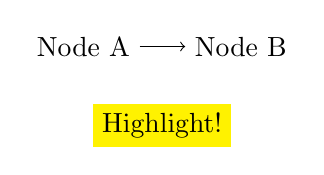
\begin{tikzpicture}
        % Node appears on slide 1
        \node<1-> (a) at (0,0) {Node A};
        
        % Node appears on slide 2
        \node<2-> (b) at (2,0) {Node B};
        
        % Arrow appears on slide 3
        \draw<3-> [->] (a) -- (b);
        
        % Highlighted on slide 4
        \node<4> [fill=yellow] at (1,-1) {Highlight!};
    \end{tikzpicture}
\end{frame}

% Using visible on style
\begin{frame}{TikZ Visible On}
    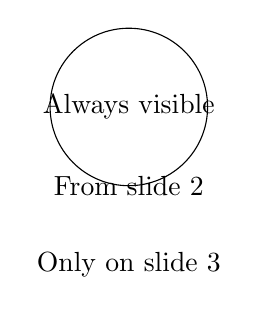
\begin{tikzpicture}
        \node[visible on=<1->] {Always visible};
        \node[visible on=<2->] at (0,-1) {From slide 2};
        \node[visible on=<3>] at (0,-2) {Only on slide 3};
        
        % Alternative syntax
        \draw[visible on=<2-3>] (0,0) circle (1cm);
    \end{tikzpicture}
\end{frame}
\end{lstlisting}

\subsection{\textbackslash temporal Command}

The \verb|\temporal| command provides three alternatives:
\begin{lstlisting}
\temporal<2>{Before}{During}{After}
\temporal<2-4>{Initial}{Highlighted}{Final}

% Example with formatting
\temporal<2-3>
    {\color{gray}Text}     % Before slides 2-3
    {\color{red}\textbf{Text}}  % During slides 2-3
    {\color{blue}Text}      % After slide 3
\end{lstlisting}

\subsection{Handout Mode}

\begin{lstlisting}
% In preamble
\documentclass[handout]{beamer}

% Handout-specific content
\only<beamer>{This only appears in presentation mode}
\only<handout>{This only appears in handout mode}

% Selecting specific slides for handout
\only<beamer:1-3|handout:2>{Slides 1-3 in beamer, slide 2 in handout}
\end{lstlisting}

\section{Part 2: Overlays in Regular LaTeX Documents}

\subsection{TikZ Overlays and Layers}

TikZ provides powerful overlay capabilities in regular documents:

\subsubsection{Basic TikZ Overlays}
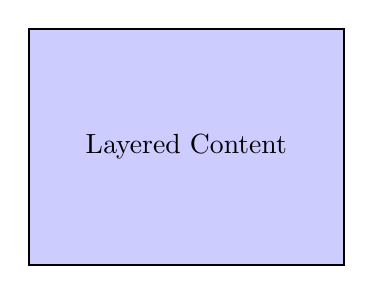
\begin{tikzpicture}
    % Background layer
    \fill[blue!20] (0,0) rectangle (4,3);
    
    % Middle layer
    \draw[thick] (0,0) rectangle (4,3);
    
    % Foreground layer
    \node at (2,1.5) {Layered Content};
\end{tikzpicture}

\begin{lstlisting}
\begin{tikzpicture}[remember picture,overlay]
    % Draw on top of the page
    \draw[red,thick] (current page.north west) -- (current page.south east);
    \node[rotate=45] at (current page.center) {\Huge DRAFT};
\end{tikzpicture}
\end{lstlisting}

\subsubsection{TikZ Layers}
\begin{lstlisting}
\pgfdeclarelayer{background}
\pgfdeclarelayer{foreground}
\pgfsetlayers{background,main,foreground}

\begin{tikzpicture}
    \begin{pgfonlayer}{background}
        \fill[yellow!30] (0,0) rectangle (3,2);
    \end{pgfonlayer}
    
    \draw (0,0) rectangle (3,2);
    \node at (1.5,1) {Main layer};
    
    \begin{pgfonlayer}{foreground}
        \draw[red,thick] (0,0) -- (3,2);
    \end{pgfonlayer}
\end{tikzpicture}
\end{lstlisting}

\subsection{Spacing Overlays with \textbackslash phantom}

\subsubsection{Basic phantom}
Text with phantom: X\phantom{invisible}X

Text without phantom: XX

\begin{lstlisting}
% Horizontal spacing
Before\phantom{invisible text}After

% Vertical spacing
Line 1\\
\vphantom{\Huge Big}Line 2\\
Line 3
\end{lstlisting}

\subsubsection{Mathematical phantoms}
\[
    \frac{a}{\phantom{b}c} \quad \text{vs} \quad \frac{a}{c}
\]

\subsection{Text Overlapping Commands}

\subsubsection{\textbackslash llap, \textbackslash rlap, \textbackslash clap}

Right overlap: Text\rlap{\ overlapping}\ continues

Left overlap: Text\ \llap{overlapping\ }continues

Center overlap: Text\clap{\ overlapping\ }continues

\begin{lstlisting}
% Right overlap (zero width, extends right)
Normal\rlap{\color{red} Overlapped} Text

% Left overlap (zero width, extends left)
Normal \llap{\color{blue}Overlapped}Text

% Center overlap
Normal\clap{\rule{3cm}{0.5pt}}Text
\end{lstlisting}

\subsection{The overpic Package}

\begin{lstlisting}
\usepackage{overpic}

% Basic usage (requires an image file)
\begin{overpic}[width=5cm,grid,tics=10]{example-image}
    \put(20,30){\color{red}Label 1}
    \put(60,70){\color{blue}\Large Label 2}
    \put(10,10){\rotatebox{45}{Rotated}}
\end{overpic}
\end{lstlisting}

% Example with placeholder
\fbox{%
\begin{overpic}[width=5cm,height=3cm]{example-image-a}
    \put(20,50){\color{red}\textbf{Overlay Text}}
    \put(70,20){\color{blue}$E=mc^2$}
\end{overpic}%
}

\subsection{The textpos Package}

\begin{lstlisting}
\usepackage[absolute,overlay]{textpos}
\setlength{\TPHorizModule}{1cm}
\setlength{\TPVertModule}{1cm}

% Absolute positioning
\begin{textblock}{5}(10,5)
    This text block is 5cm wide, positioned at (10cm,5cm)
\end{textblock}

% Overlay example
\begin{textblock}{3}[0.5,0.5](8,4)
    \colorbox{yellow}{Floating Box}
\end{textblock}
\end{lstlisting}

% Demonstration
\begin{textblock}{4}(12,22)
    \fbox{\parbox{3.5cm}{This is a floating text block positioned absolutely on the page.}}
\end{textblock}

\subsection{Using tikzmark}

\begin{lstlisting}
\usepackage{tikz}
\usetikzlibrary{tikzmark,calc}

% Mark positions in text
This is \tikzmark{start}important\tikzmark{end} text.

% Draw connections
\begin{tikzpicture}[remember picture,overlay]
    \draw[red,thick]
        ([yshift=2pt]pic cs:start) rectangle ([yshift=-2pt]pic cs:end);
\end{tikzpicture}
\end{lstlisting}

Example: Mark \tikzmark{a}this\tikzmark{b} and \tikzmark{c}that\tikzmark{d}.

\begin{tikzpicture}[remember picture,overlay]
    \draw[blue,thick,<->] ([yshift=-3pt]pic cs:a) -- ([yshift=-3pt]pic cs:c);
    \node[above] at ($(pic cs:a)!0.5!(pic cs:c)$) {\tiny connected};
\end{tikzpicture}

\subsection{The animate Package}

\begin{lstlisting}
\usepackage{animate}

% Create frame-by-frame animation
\begin{animateinline}[controls,loop]{2}
    % Frame 0
    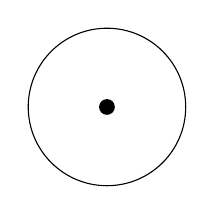
\begin{tikzpicture}
        \draw (0,0) circle (1);
        \fill (0,0) circle (0.1);
    \end{tikzpicture}
\newframe
    % Frame 1
    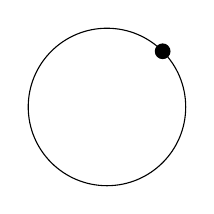
\begin{tikzpicture}
        \draw (0,0) circle (1);
        \fill (45:1) circle (0.1);
    \end{tikzpicture}
\newframe
    % Frame 2
    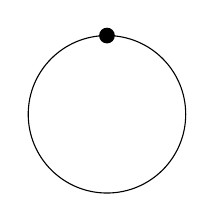
\begin{tikzpicture}
        \draw (0,0) circle (1);
        \fill (90:1) circle (0.1);
    \end{tikzpicture}
\end{animateinline}
\end{lstlisting}

\subsection{Multi-layer Diagrams}

\subsubsection{Complex Layer Example}

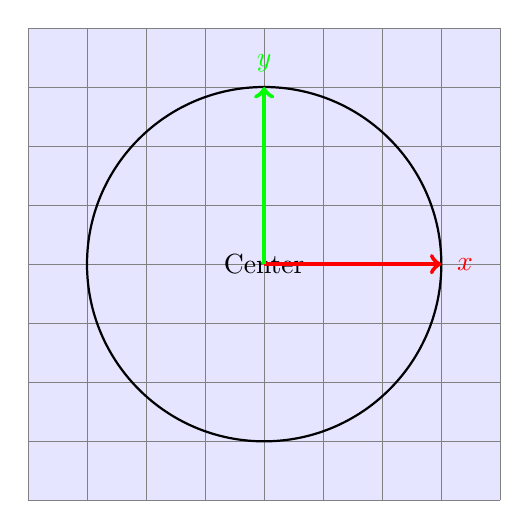
\begin{tikzpicture}[scale=1.5]
    % Define layers
    \pgfdeclarelayer{background}
    \pgfdeclarelayer{foreground}
    \pgfsetlayers{background,main,foreground}
    
    % Background
    \begin{pgfonlayer}{background}
        \fill[blue!10] (-2,-2) rectangle (2,2);
        \draw[help lines,step=0.5] (-2,-2) grid (2,2);
    \end{pgfonlayer}
    
    % Main layer
    \draw[thick] (0,0) circle (1.5);
    \node at (0,0) {Center};
    
    % Foreground
    \begin{pgfonlayer}{foreground}
        \draw[red,ultra thick,->] (0,0) -- (1.5,0);
        \draw[green,ultra thick,->] (0,0) -- (0,1.5);
        \node[red] at (1.7,0) {$x$};
        \node[green] at (0,1.7) {$y$};
    \end{pgfonlayer}
\end{tikzpicture}

\section{Advanced Techniques}

\subsection{Combining Multiple Overlay Methods}

\begin{lstlisting}
% Complex overlay with TikZ and textpos
\begin{textblock}{5}(10,15)
    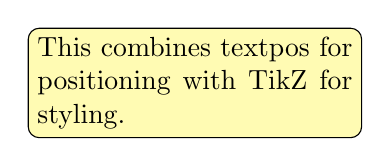
\begin{tikzpicture}
        \node[draw,rounded corners,fill=yellow!30] {
            \parbox{4cm}{
                This combines textpos for positioning
                with TikZ for styling.
            }
        };
    \end{tikzpicture}
\end{textblock}

% Overlay with mathematical content
\[
    \underbrace{a + b}_{\text{\clap{sum}}} = 
    \overbrace{c}^{\text{\rlap{result}}}
\]
\end{lstlisting}

\subsection{Creating Watermarks}

\begin{lstlisting}
% Page-wide watermark
\usepackage{eso-pic}
\AddToShipoutPictureBG{%
    \begin{tikzpicture}[remember picture,overlay]
        \node[rotate=45,scale=10,text opacity=0.1]
            at (current page.center) {DRAFT};
    \end{tikzpicture}%
}
\end{lstlisting}

\subsection{Overlay Effects in Tables}

\begin{lstlisting}
\begin{tabular}{|c|c|c|}
    \hline
    A & B & C \\
    \hline
    1 & 2 & 3 \\
    \hline
    \multicolumn{2}{|c|}{\cellcolor{yellow}Merged} & 6 \\
    \hline
\end{tabular}

% With TikZ overlay
\begin{tikzpicture}[remember picture]
    \node[inner sep=0pt] (table) {
        \begin{tabular}{|c|c|c|}
            \hline
            A & B & C \\
            \hline
            1 & \tikzmark{cell}2 & 3 \\
            \hline
        \end{tabular}
    };
    \begin{scope}[overlay]
        \draw[red,thick,->] (cell) -- ++(1,0.5) 
            node[right] {Important!};
    \end{scope}
\end{tikzpicture}
\end{lstlisting}

\section{Best Practices}

\subsection{Beamer Overlays}
\begin{enumerate}
    \item Use \verb|\pause| for simple sequential reveals
    \item Prefer \verb|\only| when content should not affect spacing
    \item Use \verb|\uncover| to maintain consistent layout
    \item Apply \verb|[<+->]| to lists for automatic incrementing
    \item Consider handout mode when designing overlays
    \item Test presentations with different overlay densities
\end{enumerate}

\subsection{Document Overlays}
\begin{enumerate}
    \item Use \verb|remember picture,overlay| for page-wide effects
    \item Define layers for complex diagrams
    \item Combine \verb|\phantom| with math for alignment
    \item Use \verb|textpos| for absolute positioning needs
    \item Apply \verb|tikzmark| for connecting distant elements
    \item Test PDF compatibility when using animations
\end{enumerate}

\section{Troubleshooting}

\subsection{Common Issues}
\begin{itemize}
    \item \textbf{Overlapping content}: Check layer ordering
    \item \textbf{Missing overlays}: Compile twice for TikZ overlays
    \item \textbf{Animation not working}: Ensure PDF viewer supports JavaScript
    \item \textbf{Textpos positioning}: Verify module settings
    \item \textbf{Beamer handout}: Use mode-specific commands
\end{itemize}

\section{Conclusion}

This guide has covered comprehensive overlay techniques for both beamer presentations and regular LaTeX documents. From simple reveals to complex multi-layer diagrams, these tools provide powerful ways to create dynamic and visually appealing documents.

Key takeaways:
\begin{itemize}
    \item Beamer provides specialized overlay commands for presentations
    \item TikZ offers flexible layering for both document types
    \item Multiple packages can be combined for advanced effects
    \item Always consider the output format and viewer capabilities
\end{itemize}

\appendix
\section{Quick Reference}

\subsection{Beamer Overlay Commands}
\begin{tabular}{ll}
    \textbf{Command} & \textbf{Purpose} \\
    \hline
    \verb|\pause| & Simple sequential reveal \\
    \verb|\only<n>{...}| & Show only on slide(s) n \\
    \verb|\uncover<n>{...}| & Reveal on slide(s) n (space reserved) \\
    \verb|\visible<n>{...}| & Make visible on slide(s) n \\
    \verb|\invisible<n>{...}| & Make invisible on slide(s) n \\
    \verb|\alt<n>{A}{B}| & Show A on n, B otherwise \\
    \verb|\temporal<n>{A}{B}{C}| & A before n, B during n, C after \\
    \verb|\alert<n>{...}| & Highlight on slide(s) n \\
\end{tabular}

\subsection{Regular Document Overlay Tools}
\begin{tabular}{ll}
    \textbf{Package/Command} & \textbf{Purpose} \\
    \hline
    TikZ layers & Multi-layer drawings \\
    \verb|\phantom{...}| & Invisible space reservation \\
    \verb|\rlap{...}|, \verb|\llap{...}| & Zero-width overlaps \\
    overpic & Overlay on images \\
    textpos & Absolute positioning \\
    tikzmark & Mark and connect points \\
    animate & PDF animations \\
\end{tabular}

\end{document}